\documentclass[journal]{IEEEtran}

\usepackage{mathptmx}
\usepackage[T1]{fontenc}
\usepackage{textcomp}
\usepackage{amsmath,amssymb}
\usepackage{graphicx}
\usepackage{tikz}
\usetikzlibrary{arrows.meta,positioning,fit,calc}
\usepackage{booktabs}
\usepackage{tabularx}
\usepackage{multirow}
\usepackage{array}
\usepackage{cite}
\usepackage{url}
\usepackage{balance}

\hyphenation{Bullet-Git Gas-Town Omni-gent Deep-Seek work-tree}

\begin{document}

\title{Bullet Farm: A Transaction Processor for Verified Multi-Agent Software Engineering}

\author{Bullet~Farm~Maintainers%
\thanks{Placeholder authorship for this preprint. Named authors will be supplied before an arXiv upload. Affiliation: the Bullet Farm split family (public hub, kernel, BulletGit, and operations portal). This document is not a release receipt, installer, or benchmark result.}%
}

\markboth{Bullet Farm Technical Preprint, August 2026}{Bullet Farm Maintainers: Transaction Processor for Multi-Agent Software Engineering}

\maketitle

\begin{abstract}
Coding agents are proliferating as chat loops, plugin kernels, and meta-wrappers around existing CLIs. The scarce resource is not another persona or sandbox flag. It is a correct concurrent \emph{software-change transaction}: who may mutate an exact repository subject, which incarnation owns that write, what evidence names that subject, and whether an ambiguous remote effect may be retried. Bullet Farm is a local-first transaction processor for software changes and model cognition. Models may propose typed patches. They cannot grant write, verification, or merge authority. This preprint inventories the architecture and the exact component receipts that exist on 2026-08-25, and it compares that contract with Gas Town~/~Gas City, DeepSeek Harness, Databricks Omnigent, and the broader coding-agent landscape. Many Kernel, BulletGit, and Portal machines now have commit-bound component proofs. The connected five-plane product and every family release gate remain blocked. The paper claims a stronger systems contract, not measured superiority.
\end{abstract}

\begin{IEEEkeywords}
Multi-agent software engineering, transaction processing, Git isolation, evidence binding, authority fencing, coding agents, verification.
\end{IEEEkeywords}

\section{Introduction}
\label{sec:intro}

The last two years produced a crowded market of coding agents: protocol-grade CLIs, IDE wrappers, hosted pull-request bots, research SWE loops, multi-agent orchestrators, plugin kernels, and meta-harnesses that wrap the previous categories~\cite{claudeCode,codexCli,cursorAcp,antigravity,gastownReadme,dshReadme,omnigentBlog}. Those systems differ in user experience and in how much of the model loop they own. They largely agree on an implicit completion rule: if a session looks done, a terminal is idle, a process exited zero, or a pull request opened, the work is complete.

That rule fails under concurrency. Public Gas Town and Gas City issues show the same family of faults repeating under load: two agents share one working tree and clobber uncommitted edits~\cite{gascity1181}; a timeout after a server-side commit mints duplicate live workflows and three writers enter one checkout~\cite{gascity5511}; a background \texttt{git checkout} against the town-root \texttt{.git} deletes operational files~\cite{gastown4094}; a dead tmux session is treated as live ownership and drives hundreds of respawns~\cite{gastown742}. Those reports are not a verdict that Gas Town is a weak product. They are evidence that a role/session orchestrator is the wrong abstraction for adversarial multi-writer Git~\cite{gastownAudit}.

DeepSeek Harness and Omnigent improve different layers. DeepSeek treats every capability---model, tools, sandbox, session, and UI---as a Cordis plugin and makes the append-only session log the source of model-visible context~\cite{dshArch,dshSite}. Omnigent sits \emph{above} Claude Code, Codex, Cursor, and other CLIs, adding OS sandboxes, an L7 credential proxy, contextual policies, and live collaboration~\cite{omnigentReadme,omnigentBlog,omnigentPolicies}. Both are real advances. Neither binds write authority to an incarnation-fenced Attempt, evidence to an exact Candidate, or remote integration to a reconciled effect receipt. A plugin swap or a wrapped harness can still let the model run \texttt{git}.

Bullet Farm inverts the authority model~\cite{bulletOverview,adr0001}. The law is compact:

\begin{quote}
Many agents may reason. Multiple isolated Variants may compete. Exactly one incarnation-fenced Attempt may write within each Variant. Every consequential external mutation is brokered. Every proof names its exact subject. The repository remains sovereign.
\end{quote}

The contribution of this preprint is threefold. First, it states that law as a five-plane transaction, not as a prompt convention (Section~\ref{sec:arch}). Second, it shows why Git itself is the deepest missing substrate and how BulletGit answers a closed list of Git failure classes (Sections~\ref{sec:failures} and~\ref{sec:bulletgit}). Third, it reports \emph{exactly} what is implemented as of the 2026-08-25 closure reconciliation---component receipts versus blocked product gates---so a reader cannot confuse a green crate test with a release (Section~\ref{sec:inventory}). Tables~\ref{tab:authority} and~\ref{tab:git} compare authority and Git bindings. Table~\ref{tab:resolve} maps each failure class to a rule and to an honest implementation status.

This paper does not claim that Bullet Farm is faster, cheaper, or more autonomous than any named system. No public comparison is valid until the same receipt-bearing corpus runs on pinned upstream commits~\cite{bulletSnapshot}. The previous separately produced IEEE draft recorded that Bullet Farm had not been implemented~\cite{potentialDraft}. That sentence is now false for many components and still true for the connected product.

\section{A Taxonomy of Coding Agents}
\label{sec:taxonomy}

Treating ``coding agents'' as one category hides the authority question. We distinguish six families by \emph{who writes the repository} and \emph{what signal is allowed to mean done}.

\subsection{Protocol-Grade Single Agents}

Claude Code (bidirectional stream JSON), Codex (App Server JSON-RPC over stdio JSONL), Cursor (Agent Client Protocol), and Google Antigravity (\texttt{agy} structured headless mode) are the four V1 adapter targets~\cite{adr0001,claudeCode,codexCli,cursorAcp,antigravity,acpSpec}. On 2026-08-25, sanitized local probes observed Claude Code 2.1.243, Codex CLI 0.149.1, Cursor Agent 2026.08.11-e8db854, and \texttt{agy} 1.1.19. Those observations are inventory, not certification. Cursor's required ACP entry point remained \texttt{UNKNOWN} on that host; print/stream-JSON modes must not be substituted~\cite{adr0001}. Each of these products is a capable single-agent harness. The model, or a tool the model invoked, writes the workspace. A ``plan'' flag or a vendor sandbox is defense in depth, not a foreign write gateway.

\subsection{IDE and CLI Wrappers}

Aider, Cline, Continue, Goose, and Roo Code wrap an editor or terminal around one or more models~\cite{aider,cline,continue,goose,roo}. They differ in UX, MCP adoption~\cite{mcpSpec}, and how much Git they automate. They share the user's checkout as the writable world. Isolation, if any, is a worktree, a subdirectory, or an honor-system ignore list.

\subsection{Research SWE Loops}

OpenHands, SWE-agent, Agentless, and AutoCodeRover optimize for SWE-bench-style issue resolution~\cite{openhands,yang2024sweagent,agentless,autocoderover}. Their contribution is the agent--computer interface and the evaluation harness. Completion is a resolved issue or a passing hidden test, not a protected integration onto a sovereign default branch under an independent attestor.

\subsection{Hosted Change Agents}

GitHub Copilot's coding agent, Jules, Devin, and Kiro accept a task and return a pull request or a hosted workspace~\cite{copilotAgent,jules,devin,kiro}. The PR is the product. That is a legitimate remote-collaboration contract. It is not an incarnation-fenced local transaction: retries, reviewer independence, and evidence staleness after rebase are delegated to the host's merge queue and to human review.

\subsection{Orchestrators}

Gas Town is a Go workspace manager for many Claude, Codex, Copilot, Gemini, or Cursor agents~\cite{gastownReadme,gastownV121}. It persists work in git-backed \emph{hooks} (worktrees), coordinates via Beads/Dolt, requires tmux 3.0+ for \texttt{gt up}, and lands work through a Bors-style Refinery~\cite{bors}. Roles---Mayor, Witness, Deacon, polecat, Refinery---are operationally legible. Additional product machinery is easy to underestimate: convoys bundle beads; molecules instantiate TOML formulas; a three-tier watchdog (Witness, Deacon, Dogs) patrols health; a scheduler caps polecat dispatch to avoid provider 429s; Seance recovers predecessor session logs; Wasteland federates towns over DoltHub~\cite{gastownReadme}. Gas City generalizes the same factory into Agent, Bead, Formula, Rig, Pack, and Event, with typed run/session APIs, warm projections, formula-v2 retry/fan-out/drain controls, degraded storage outcomes, and release artifacts with checksums, SBOMs, and attestations in v1.4.1~\cite{gascityV141,gascityMain,bulletSnapshot}. The product leverage is real. The authority model is not: liveness is a terminal multiplexer, isolation is a worktree or an optional pack script, and the fleet can be the merge authority. Bullet Farm should be measured against those product properties---durable work, role flexibility, fan-out receipts, provider plurality, health reconciliation, and release evidence---not against a cartoon of ``tmux and vibes''~\cite{bulletSnapshot}.

\subsection{Plugin Kernels}

DeepSeek Harness (\texttt{dsh}) is a developer-preview agent runtime whose doctrine is ``everything is a plugin''~\cite{dshReadme,dshSite}. Cordis mounts model adapters, tools, sandboxes, storage, loops, scheduling, and the UI into one context~\cite{cordis,dshArch}. A running instance is a plugin tree composed from bundles and ordered patches. The session log is the source of model-visible context: anything the model sees must be reconstructable from that log. A turn is zero or more steps; each step is one model request plus the tools it calls; \texttt{agent/pre-step} may rewrite or reject claimed messages; tool execution is a \texttt{pre-execute}/\texttt{execute}/\texttt{post-execute} waterfall~\cite{dshArch}. Standard mode gives the model a file editor, a shell, search, skills, and subagents; Code mode lets the model orchestrate tool rounds in TypeScript; Minimal mode keeps bash and \texttt{str\_replace\_editor}; Creator mode inspects the runtime to author presets~\cite{dshSite}. Experimental Agent Teams add a roster, task board, and mailbox over continuable subagents. This is an excellent composition kernel for a \emph{single} agent product. It is not a transaction kernel. Filesystem and subprocess providers share one execution world, so pointing them at a remote sandbox moves Bash and PTY together---and the model still writes files. A durable session event is not a Candidate.

\subsection{Meta-Harnesses}

Omnigent is an open-source meta-harness, with a Databricks-operated deployment, that wraps Claude Code, Codex, Cursor, OpenCode, Hermes, Pi, Antigravity, and custom YAML agents~\cite{omnigentReadme,omnigentV010,omnigentBlog}. A runner exposes a uniform session API. A server stores policies and sharing. Native Linux wrappers use bubblewrap; macOS uses seatbelt; an L7 egress proxy can attach credentials so the sandbox never holds the real token~\cite{omnigentPolicies}. That credential-proxy design is one of the strongest OS-isolation stories in this survey. Native terminal wrappers still require tmux. The wrapped harness still performs Git. A policy can deny, transform, or pause a tool call; it cannot mint a Candidate or invalidate evidence when the branch moves.

\section{Recurring Failure Classes}
\label{sec:failures}

The issue corpus and the Git documentation converge on a small set of missing \emph{bindings}~\cite{gastownAudit,gitdocs,gitRole}. A binding is a rule that makes a class of silent success impossible. Role names, dashboards, and sandboxes do not substitute. Table~\ref{tab:authority} summarizes how the surveyed systems bind---or fail to bind---write, completion, evidence, integration, and liveness.

\begin{table*}[!t]
\caption{Authority bindings. ``Typical harness'' is the Claude Code / Codex / Cursor / Antigravity single-agent pattern~\cite{adr0001}.}
\label{tab:authority}
\centering
{\scriptsize
\begin{tabular}{@{}p{0.13\textwidth}p{0.13\textwidth}p{0.12\textwidth}p{0.13\textwidth}p{0.13\textwidth}p{0.14\textwidth}p{0.12\textwidth}@{}}
\toprule
System & Who writes the repo & Isolation & Completion signal & Evidence subject & Integration authority & Liveness oracle \\
\midrule
Bullet Farm (designed) & \texttt{bullet-gitd} only & Private clone, no worktree & Candidate + independent Evidence + forge receipt + observation & $\{\mathrm{base},\mathrm{head},\mathrm{tree},\mathrm{patch},\mathrm{env}\}$ & Jeryu/GitHub required checks; attestor $\ne$ broker & Lease/fence; ALIVE/DEAD/UNKNOWN/CONTRADICTORY \\
Bullet Farm (implemented) & Production write refused & Dissociate clone code exists; not reachable online & \texttt{PENDING}$\rightarrow$\texttt{UNKNOWN}/\texttt{FAILED} only & One fixture E2 gate; no live subject & Local bare-forge component; Jeryu quarantined & DB-clock leases; no signed final check \\
Gas Town v1.2.1 & Agent in hook worktree & Git worktree sharing \texttt{.git} & \texttt{gt done}, convoy, Refinery merge & Gates exist; not exact-OID bound & Refinery / local merge queue & tmux session \\
Gas City v1.4.1 & Agent; implicit pool uses rig root~\cite{gascity1181} & Pack-optional worktree & Formula/run/session closure & Session and bead state & Configurable; still orchestrator-owned & Session + controller \\
DeepSeek Harness rc.2 & Model via fs/shell plugins & Sandbox plugin backend & Turn/session log & Session events (model-visible) & n/a (not a forge OS) & Agent loop \\
Omnigent v0.10.0 & Wrapped harness & OS sandbox + L7 proxy & Session / policy decision & Policy and session events & n/a (meta-harness) & tmux on native wrappers \\
Typical single-agent harness & The agent in the user checkout & Vendor sandbox flags (optional) & Model ``done'', PR, or exit 0 & Transcript or CI on a branch & Hosted PR or human merge & Process / IDE session \\
\bottomrule
\end{tabular}
}
\end{table*}

\subsection{Shared Writable Identity}

Git worktrees share one object store, one set of refs, and---unless extra machinery exists---one index and one hook namespace~\cite{gitdocs}. Gas City issue~1181 records implicit pool agents resolving every session to the rig root: two parallel slings clobber uncommitted edits~\cite{gascity1181}. Gas Town issue~4094 records background polecat operations running \texttt{git checkout} against the town-root \texttt{.git}, deleting untracked operational files such as \texttt{mayor/rigs.json} and Dolt manifests~\cite{gastown4094}. A worktree is a checkout convenience. It is not a private repository.

\texttt{git clone --reference} without \texttt{--dissociate} writes \texttt{objects/info/alternates} into a borrowed store. A later \texttt{git gc --prune=now} on the mirror can unlink objects a live workspace still names~\cite{gitdocs,potentialDraft}. CoW reflinks without a documented fallback have the same ownership question.

\subsection{Hostile Configuration and Inherited Credentials}

A repository-local or inherited Git config can install filters, aliases, include files, URL rewrites, credential helpers, hooks, and \texttt{protocol.file} transports that execute host code or exfiltrate bytes during an ordinary \texttt{checkout} or \texttt{diff}~\cite{gitdocs,gitArch}. Case-folded path collisions on a case-insensitive volume, alternate data streams, and symlink traversal are the same class: Git will write something the operator did not grant. Model-authored \texttt{git} in a process that inherited \texttt{GIT\_*}, \texttt{SSH\_AUTH\_SOCK}, or a forge token is a credential and integrity failure, not a convenience. Compile-time code---Rust \texttt{build.rs}, proc-macros, TypeScript transformers---executes before any test ``runs''~\cite{potentialDraft}. Sandboxing only the test process is insufficient. Detached HEAD, an active sequencer (\texttt{MERGE\_HEAD}, \texttt{REBASE\_HEAD}), and a dirty index shared across worktrees convert ordinary ``just commit'' steps into lost or mis-attributed work~\cite{gitdocs}.

\subsection{Control Plane in Git}

Git is a poor coordination database for renewable leases, heartbeats, quota reservations, and unsettled remote effects~\cite{gitRole,gray1981tp}. Beads-on-Dolt-in-Git is an inventive store and an operationally heavy one: install depends on Dolt, ICU, and \texttt{bd}, and writer-deadlock classes appear under load~\cite{gastownReadme,gascity5511}. Putting the live ledger in the same bytes the agents edit couples control-plane availability to repository mutation.

\subsection{Inferred Completion and Unsafe Liveness}

Gas Town's problems-view calls a dead agent a ``Zombie: Dead tmux session''~\cite{gastownReadme}. Issue~742 shows the failure: a dead session left work claimed and drove 687 respawns in 24~h~\cite{gastown742}. A timeout after Dolt committed server-side is classified transient and retried, yielding three complete workflows from one \texttt{gc sling}~\cite{gascity5511}. Hosted agents treat PR-opened as done. Plugin kernels treat turn-end as done. In every case, transport success is painted as domain success.

\subsection{Evidence Not Bound to an Exact Subject}

A green CI result that names a branch, a worktree path, or a session ID is not evidence about a rebase, a repair commit, or a merge-group composition. Ordinary Git commits have no stable Change identity across rewrite~\cite{gitdocs,jjvcs}. After the branch moves, yesterday's green is a different subject. Merge queues that do not invalidate overlapping evidence create silent stale-green admission; queues that invalidate every queued candidate recreate a livelock when arrival rate exceeds verification time~\cite{potentialDraft}.

\subsection{Destruction Without Preservation}

Cleanup, GC, polecat reuse, and ``nuke'' operations that target a name, path, or inferred age destroy the only copy of uncommitted work~\cite{gastown4094,gastownAudit}. Preservation must bind an exact incarnation and a sealed artifact \emph{before} deletion eligibility.

\section{Bullet Farm Architecture}
\label{sec:arch}

Bullet Farm is a split family: a public hub (\texttt{bullet-farm}), a control-plane kernel, a Git capability daemon, and a projection-only portal~\cite{bulletOverview}. Jeryu is the source forge and the mandatory local effect adapter. GitHub is a separately configured effect adapter, never source authority.

\subsection{The Software-Change Transaction}

\begin{equation}
\begin{aligned}
&\mathrm{Mission}\rightarrow\mathrm{GraphRevision}\rightarrow\mathrm{Variant}\rightarrow\mathrm{Attempt}\\
&\rightarrow\mathrm{Proposal}\rightarrow\mathrm{Candidate}\rightarrow\mathrm{Evidence}\\
&\rightarrow\mathrm{Effect}\rightarrow\mathrm{Integration}\rightarrow\mathrm{Observation}.
\end{aligned}
\end{equation}

A Mission is a durable objective plus constraints. A Graph Revision is an immutable package decomposition. A Variant is one hypothesis with an immutable role, routing, context, and configuration snapshot. An Attempt is one execution incarnation under a unique lease and a never-reused fence. A Proposal is typed patch data. A Candidate is a provenance-bound immutable phenotype created only by BulletGit. Evidence is an independently reproduced result over that exact Candidate and admitted gate definitions. An Effect is a brokered remote mutation with read-back. Integration is protected-ref admission by the forge. Observation is post-merge survival. None of those words is a prompt label. Each is a typed subject with an exact identifier~\cite{bulletOverview,bulletEvo}.

\subsection{Five Trust Planes}

\begin{figure}[!t]
\centering
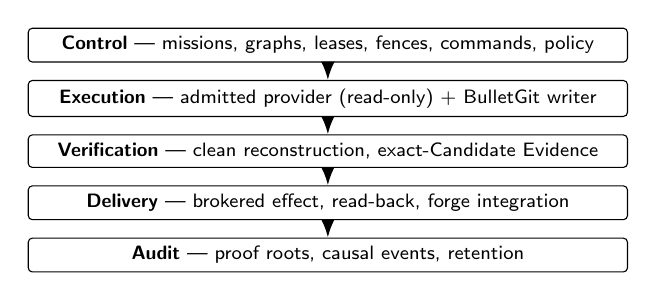
\begin{tikzpicture}[
  font=\scriptsize\sffamily,
  box/.style={draw, rounded corners=1.5pt, align=center, inner sep=3pt, text width=7.4cm},
  arr/.style={-{Latex}, thick}
]
\node[box] (c) {\textbf{Control} --- missions, graphs, leases, fences, commands, policy};
\node[box, below=2.2mm of c] (e) {\textbf{Execution} --- admitted provider (read-only) + BulletGit writer};
\node[box, below=2.2mm of e] (v) {\textbf{Verification} --- clean reconstruction, exact-Candidate Evidence};
\node[box, below=2.2mm of v] (d) {\textbf{Delivery} --- brokered effect, read-back, forge integration};
\node[box, below=2.2mm of d] (a) {\textbf{Audit} --- proof roots, causal events, retention};
\draw[arr] (c) -- (e);
\draw[arr] (e) -- (v);
\draw[arr] (v) -- (d);
\draw[arr] (d) -- (a);
\end{tikzpicture}
\caption{Five trust planes. A plane may consume only grants addressed to its principal. Portal and any evolutionary optimizer are projections or requestors, never mutation credentials~\cite{adr0003}.}
\label{fig:planes}
\end{figure}

ADR~0003 separates control, execution/repository write, independent verification, effect/attestation/integration, and observation/audit~\cite{adr0003}. Compromise of the portal, a provider, or a broker must not manufacture independent evidence. One-host V1 uses distinct OS identities; distributed mode later uses distinct workload identities. The evolutionary control document defines roles as capability envelopes---Planner, Implementer, Critic, Verifier, Effect broker---not as personas that carry credentials~\cite{bulletEvo}. Online learning, larger councils, and distributed execution are Phase~9--10 and are out of V1~\cite{bulletEvo}.

\subsection{Three Sovereign Truths}

A common instinct is to put missions, leases, and evidence into Git because the product is about Git. That collapses two badly matched stores~\cite{gitRole}. Bullet Farm splits canonical truth:

\begin{itemize}
\item \textbf{Kernel ledger} (SQLite WAL today; PostgreSQL is a refused scaffold~\cite{kernelArch}) owns mutable authority: leases, fences, commands, policy snapshots, outbox, event log.
\item \textbf{BulletGit} owns immutable engineering subjects: Changes, Candidates, checkpoints, journals, proof roots.
\item \textbf{Forge} (Jeryu, optionally GitHub) owns remote refs, required checks, and the merged target SHA.
\end{itemize}

Cross-boundary values come from generated \texttt{bullet-wire} contracts: RFC~8785 canonical JSON, domain-separated BLAKE3, full 256-bit IDs, algorithm-tagged Git OIDs, and PASETO v4.public envelopes~\cite{rfc8785,paseto,bulletClosure}. Prose and TypeScript types do not define the wire.

\subsection{Providers Propose}

ADR~0001 is the execution-mode decision~\cite{adr0001}. Every provider turn is read-only inside a private workspace generation. The only write input is a validated \texttt{PatchProposal}: schema identity, producing Attempt, base checkpoint, per-path preimages, and policy-admitted \texttt{gate\_ids}. Provider text such as \texttt{tests\_to\_run} or a shell command is never argv. Runner resolves gate IDs through a trusted catalog. Zero tests, timeout, skipped, flaky, unsupported, and \texttt{UNKNOWN} never equal \texttt{PASS}. At most two bounded repair turns may see typed gate results.

Public mutations use authenticated \texttt{POST /v1/commands}, initially return \texttt{202 PENDING}, and reconcile through \texttt{PENDING}$\mid$\texttt{APPLIED}$\mid$\texttt{VERIFIED}$\mid$\texttt{FAILED}$\mid$\texttt{UNKNOWN}~\cite{bulletClosure}. Transport success never implies verification. The Portal renders only those phases and treats watermark mismatch, sequence gaps, and timeouts as \texttt{UNKNOWN} or \texttt{STALE}, never as an empty success list~\cite{portalArch}.

\subsection{Why the Bindings Are the Product}

Other systems can copy a role name in a week. They cannot copy a binding without changing what an agent is allowed to \emph{be}. A Mayor that still infers liveness from tmux is a persona. A fence that is checked inside the ledger transaction at the effects gateway is a binding. A plugin that swaps the filesystem provider is composition. A daemon that is the only process allowed to apply a scoped patch is a binding. A contextual policy that pauses a tool call is governance. An Evidence record that becomes invalid when \texttt{head} moves is a binding.

That is the source of leverage. As models improve, a harness that lets the model write Git gets more destructive more quickly. A transaction processor that lets the model propose gets more useful more quickly, because the same fence, Candidate, and verifier contracts apply to a weaker economy model and to a frontier council. The evolutionary document states the same rule for search: hard constraints are filters, never terms a high score may offset, and the optimizer cannot see or learn away the safety envelope~\cite{bulletEvo}. V1 records routing provenance and does not learn online.

\subsection{A Worked \#5511-Class Fault}

Issue~5511 is the canonical timeout-after-commit race~\cite{gascity5511,potentialDraft}. Under load, \texttt{bd create --graph} is killed at the runner deadline after Dolt has already committed. The client sees a timeout, classifies it transient, and re-applies. The result is three live workflows and three writers in one checkout.

Bullet Farm's designed handling is mechanical:

\begin{enumerate}
\item Graph materialization is one serializable insert keyed by content hash. A replay returns the existing graph; it does not mint a sibling.
\item The command that requested materialization is recorded with an idempotency key. An ambiguous timeout becomes \texttt{UNKNOWN}, not a retry.
\item A resolver may adopt a remote or ledger subject only when its identity equals this Attempt's desired state. Otherwise the subject is \texttt{ORPHANED} and quarantined.
\item Even if two Attempts exist, each requires its own never-reused fence and its own private clone. They cannot share a cwd or a \texttt{.git}.
\item A writer that outlives its lease cannot push, comment, or settle: the fence is presented at the effects gateway and rejected inside the ledger transaction.
\end{enumerate}

Items~2 and the lease/fence machine have component proofs. Item~1 is specified and is not a live path at HEAD. The point of the walkthrough is not to claim the incident is closed in production. It is to show that the missing primitive is identity-exact adoption under ambiguity, not a smarter Mayor prompt.

\subsection{Evidence Tiers}

Writer output cannot satisfy an independent tier~\cite{adr0001,bulletEvo}. The designed ladder is:

\begin{itemize}
\item E0 --- untrusted provider or author claim;
\item E1 --- writer-visible gates on the author's workspace;
\item E2 --- clean independent reconstruction of the exact Candidate;
\item E3 --- hidden or historical holdout, plus hostile suites the author cannot weaken;
\item E4 --- human review.
\end{itemize}

The implemented verifier produces typed E2-shaped results for one fixture gate over exact base/head/tree subjects~\cite{bulletClosure}. Multi-gate aggregation, executable-digest admission, and E3 holdout custody remain open. That is the correct partial result: the identity rule exists before the gauntlet is populated.

\section{BulletGit: The Missing Substrate}
\label{sec:bulletgit}

Models and harnesses commoditize. An agent-first source-control substrate that understands authority, change identity, proof, lineage, and protected integration does not~\cite{gitRole}. BulletGit is that substrate. \texttt{bullet-gitd} is the sole writer of the private workspace~\cite{gitArch}. Pack protocol, refs, and protected updates remain ordinary Git at the forge.

\subsection{Private Clone, Not a Worktree}

Workspaces never clone the operator's source tree directly. A bare mirror is created or fetched under an exclusive lock. The private clone runs
\begin{center}
\texttt{git clone --reference-if-able <mirror> --dissociate}
\end{center}
while the lock is held~\cite{gitArch}. Objects may be borrowed during the copy; no \texttt{alternates} file survives. Mirror GC cannot corrupt a live workspace. Immediately after clone, \texttt{origin} is removed, \texttt{credential.helper} is emptied, \texttt{GIT\_ASKPASS} points at a deny script, and \texttt{GIT\_SSH\_COMMAND=false}. A model-issued push has no destination and no authenticator.

A \texttt{.git} \emph{file}---the on-disk shape of a worktree---is \texttt{WORKTREE\_FORBIDDEN}. Sequencer files at checkpoint time are \texttt{SEQUENCER\_ACTIVE}. Checkpoints run \texttt{git write-tree} against a temporary \texttt{GIT\_INDEX\_FILE}, never the live index.

\subsection{Hostile-Git Refusal}

The child environment is cleared of inherited \texttt{GIT\_*} variables and rebuilt with per-workspace \texttt{HOME}/\texttt{XDG}, \texttt{GIT\_CONFIG\_NOSYSTEM=1}, and \texttt{GIT\_CONFIG\_GLOBAL=/dev/null}~\cite{gitArch}. Every invocation disables paging, hooks, credentials, filesystem monitors, and external attribute files, and passes \texttt{protocol.file.allow=never} except for the one local clone that needs file transport. Before a repository-scoped command, BulletGit parses local config with includes disabled. Command-bearing or truth-redirecting filter, alias, include, pager, URL rewrite, credential, hook, or worktree settings fail closed as \texttt{HOSTILE\_GIT\_CONFIG}. A planted clean filter behind \texttt{.gitattributes} is a required refusal test.

\subsection{Scope, Identity, Preservation}

\texttt{apply\_change} validates every path against a \texttt{ScopeGrant} before writing: Unicode NFC, no \texttt{..}, no \texttt{.git} component, no alternate data streams, no symlink traversal. Duplicate and case-folded collisions refuse the whole batch. \texttt{CandidateId} is content-derived from change, tree, and head, so two trees under one Change cannot share an identifier. \texttt{patch\_hash} is BLAKE3 of \texttt{git diff base..head}. Cleanup accepts only an opaque preservation receipt that re-verifies the sealed generation immediately before deleting exactly those bytes~\cite{gitArch}.

\subsection{Honest Production Boundary}

The public daemon constructor installs an unavailable final-authority checker. In a fresh daemon, \texttt{clone} returns \texttt{AUTHORITY\_CONTRACT\_UNAVAILABLE} before repository I/O~\cite{gitArch}. Later verbs fail \texttt{NOT\_CLONED}. The unsigned legacy token grants nothing. Production enablement still requires a published immutable \texttt{bullet-wire} tag, local PASETO verification, Kernel online reservation, and one-second operation permits. That fail-closed posture is a feature of the current tree, not a footnote.

\section{Exact Inventory: What Works Today}
\label{sec:inventory}

Table~\ref{tab:inventory} is a receipt table, not a feature list. Subjects are those recorded by the V1 closure plan immediately before this paper's source was authored~\cite{bulletClosure}. Family HEADs at that reconciliation were hub \texttt{4b93a04}, kernel \texttt{365bb5d}, BulletGit \texttt{f551736}, and portal \texttt{181cd00}. A newer commit invalidates a row until the mapped gate is replayed.

\begin{table}[!t]
\caption{Selected component receipts versus product gates (2026-08-25). \texttt{COMPLETE} means a named commit and mapped tests exist. It does not mean a release.}
\label{tab:inventory}
\centering
{\scriptsize
\begin{tabularx}{\columnwidth}{@{}>{\raggedright\arraybackslash}p{0.28\columnwidth}>{\raggedright\arraybackslash}p{0.14\columnwidth}X@{}}
\toprule
Subject & Class & Boundary \\
\midrule
Signed wire DTOs, JCS, PASETO shapes & COMPLETE & No running issuer; no immutable published tag \\
DB-clock leases, TTL $1..15$s, never-reused fence & COMPLETE & No signed final-authority mint \\
Atomic lease/command/event/outbox & COMPLETE & Public dispatch of providers/effects open \\
Four offline provider parsers (Claude, Codex, Cursor, Antigravity) & COMPLETE & Public spawn refused; no live conformance \\
Admitted fixture gate + bounded verifier transport & COMPLETE & One fixture gate; no JSON-RPC production path \\
Fail-closed \texttt{bullet-gitd} + dissociate clone + hostile-git + preservation & COMPLETE & Production \texttt{clone} refused \\
Portal CSRF/202 + \texttt{PENDING}$\rightarrow$\texttt{UNKNOWN} + SSE STALE & COMPLETE & Not packaged/embedded; 11 surfaces stay explicit UNKNOWN \\
Setup refuses schema-2 hub-only install & COMPLETE & No signed schema-3 lock or prebuilt installer \\
Two TLA+ models (lease/fence; effect ambiguity) & COMPLETE & No third formal model is a V1 gate~\cite{lamport2002tla} \\
\midrule
Five-plane \texttt{TRANSACTION\_PROOF} & BLOCKED & No signed cross-plane crash receipt at HEAD \\
Live provider / Jeryu / GitHub effects & BLOCKED & Admission and forge credentials operator-gated \\
Hub Jankurai $\ge 90$, zero hard findings & BLOCKED & Score 58; 25 hard findings \\
Family \texttt{check release} & BLOCKED & $26/26$ gates; static negative inventory \\
Evolutionary recipe archive & designed & Gated on a working transaction; not started \\
\bottomrule
\end{tabularx}
}
\end{table}

Kernel architecture is equally explicit about what the bins are not~\cite{kernelArch}. \texttt{bullet-farmd} records \texttt{PENDING} and an internal reconciler can settle known demo work only to \texttt{UNKNOWN} or unsupported kinds to \texttt{FAILED}. It cannot emit \texttt{APPLIED} or \texttt{VERIFIED}. Provider admission compares an absolute executable to a BLAKE3 digest, builds a unique mode-0700 \texttt{HOME}, copies only digest-checked OAuth files as mode~0400, and strips host \texttt{PATH}, SCM, cloud, SSH, and API secrets. Dispatch remains blocked without signed authority and audited egress: every current receipt contains those two blockers. The four provider crates are pure transcript machines. Feature-gated ``live'' tests pass by refusing spawn.

An archived live demo receipt from 2026-08-24 14:04Z exists in the family evidence bundle. HEAD policy keeps \texttt{live\_admission\_enabled=false}. That archive does not certify the current tree and does not clear a release gate~\cite{bulletRelease}.

Exactly two protocols are model-checked in TLA+ and pinned by a model lock: lease/fence/reclaim, and command/effect ambiguity under timeout~\cite{lamport2002tla,bulletClosure}. A third formal model is not a V1 gate. The implemented models must continue to encode fence monotonicity; a skeleton that omits the conflict path does not earn a deadlock-freedom claim~\cite{potentialDraft}.

The internal engineering scorecard that accompanies the closure program called the paper architecture high and the weighted ``done and actually working'' product about $26/100$. We report that number only as an operator-facing honesty check. The citable facts are the receipt rows and the blocked gates.

\section{Comparison}
\label{sec:compare}

Tables~\ref{tab:authority} and~\ref{tab:git} use pinned subjects: Gas Town v1.2.1, Gas City v1.4.1, DeepSeek Harness \texttt{dsh-v0.1.1-rc.2} (\texttt{b150a55}), Omnigent v0.10.0 (\texttt{40755dd})~\cite{bulletSnapshot,gastownV121,gascityV141,dshReadme,omnigentV010}. Empty knowledge is written \texttt{unknown}, never guessed. Bullet Farm is split into the designed contract and the implemented tree so a reader cannot promote a document into a daemon.

\begin{table*}[!t]
\caption{Git and workspace substrate. ``Impl.'' is the Bullet Farm tree at the Section~\ref{sec:inventory} subjects.}
\label{tab:git}
\centering
{\scriptsize
\begin{tabular}{@{}p{0.16\textwidth}p{0.10\textwidth}p{0.11\textwidth}p{0.12\textwidth}p{0.11\textwidth}p{0.12\textwidth}p{0.12\textwidth}@{}}
\toprule
System & Private clone & Dissociate / CoW & Hostile-Git refuse & Path scope grant & Stable Change/Candidate & Preserve-before-destroy \\
\midrule
Bullet Farm designed & required & required & required & required & required & required \\
Bullet Farm impl. & code present; production \texttt{clone} refused & \texttt{--reference-if-able --dissociate} implemented & implemented in \texttt{SafeGit} & implemented & wire-shaped IDs; provenance-complete Candidate still open & implemented locally; online settlement open \\
Gas Town / City & no (worktree / shared cwd) & not the isolation story & unknown as a kernel & optional pack scripts & bead IDs, not Candidate OIDs & reuse/reset; issue~4094 class \\
DeepSeek Harness & unknown (workspace = fs provider) & n/a & plugin policy, not Git parser & tool/sandbox policy & session IDs & session persist, not sealed generation \\
Omnigent & sandbox FS, not a private \texttt{.git} & n/a & OS + credential proxy & policy handler & session IDs & sandbox lifetime \\
Typical harness & user's checkout & rare / foot-gun if used & inherited Git config & prompt or ignore file & Git commit SHA only & leftover branches \\
\bottomrule
\end{tabular}
}
\end{table*}

The comparison is deliberately unfair to Bullet Farm on maturity and fair to everyone on bindings. Gas Town is a shipped orchestrator with years of operational texture. DeepSeek is a composable agent product. Omnigent is a collaboration and governance layer that can wrap the others tomorrow. Bullet Farm is pre-release. What the others do not have---and what makes the architecture categorically different---is the set of bindings in the first row of each table. A system can add a Mayor, a plugin, or a policy function and still retry an \texttt{UNKNOWN} push into a shared worktree.

\subsection{What We Must Not Lose From Each System}

Gas Town's factory metaphor is the right product skin for a fleet: named work, visible roles, escalation, and a merge rail an operator can watch~\cite{gastownReadme,gastownAudit}. Bullet Farm should keep those surfaces as projections over the event log, not as authority-bearing model personas. Gas City's primitive test---keep judgment out of transport, prefer primitives that remain useful as models improve---is compatible~\cite{bulletSnapshot}. The added Bullet rule is that transport success, task closure, session state, and model judgment cannot confer mutation, verification, or integration authority.

DeepSeek's session-log invariant---model-visible means logged---is the correct epistemology for a \emph{cognitive} plane~\cite{dshArch}. Bullet Farm needs the same discipline for prompts, tool schemas, and injected context. It must not use that log as repository truth. A reconstructable transcript proves what the model saw. It does not prove what landed on \texttt{main}.

Omnigent's L7 credential proxy is the correct shape for forge and provider secrets: the sandbox never holds the real token; the proxy attaches it on approved egress~\cite{omnigentBlog,omnigentPolicies}. ADR~0007 and the provider-admission crate already strip host secrets and project minimum OAuth copies~\cite{adr0007,kernelArch}. The remaining work is audited provider-only egress, not a decision to put \texttt{GH\_TOKEN} back in the child environment. Omnigent's multi-device session sharing is a collaboration product. Bullet Farm's Portal is the opposite product on purpose: a sequence-bound projection with no skip-checks affordance~\cite{portalArch}.

Typical single-agent harnesses remain the right \emph{proposal producers}. V1 GA requires conformant Claude, Codex, Cursor, and Antigravity adapters under one proposal/evidence contract~\cite{adr0001,bulletClosure}. Wrapping them (Omnigent) or replacing their loop (DeepSeek) is a different layer. Bullet Farm's layer is the transaction around them.

\subsection{Interoperability Without Authority Leakage}

ACP and MCP are emerging interoperability layers~\cite{acpSpec,mcpSpec}. They should be consumed as capability observations and tool seams, never as mutation authority. A Cursor ACP session that streams a patch is a provider transcript. An MCP server that can run \texttt{git} is a hostile tool until it is reduced to a typed proposal or an admitted gate. The same rule applies to vendor ``plan'' modes: they are useful read-only observations. They do not admit a write.

\section{Identity, Quota, and the Human Seat}
\label{sec:identity}

Gas Town's scheduler is a rate governor (\texttt{scheduler.max\_polecats}) aimed at 429s~\cite{gastownReadme}. That is necessary and not sufficient. The historical Bullet Farm identity design---still designed, not a live quota plane---names profiles with owner, authorization class, custody mode, credential generation, and health~\cite{potentialDraft,bulletEvo}. Personal CLI subscriptions stay in local custody; API and enterprise credentials use envelope encryption. Login success comes from an adapter \texttt{auth\_status} probe, never from a UI button. Quota observations are typed and ranked: official API, structured event, headers, typed limit, estimator, then \texttt{unknown}. \texttt{unknown} is never scheduled as headroom. A bounded probe reservation may convert unknown to known without scheduling bulk work on a guess.

Named human subscriptions are rate-governed to one seat-equivalent per human regardless of how many consumer logins an operator can collect. Throughput must come from \texttt{api\_credit}, \texttt{organization\_seat}, or \texttt{service\_identity}. That rule is a compliance-as-code stance, not legal advice, and it is not enforced in the current kernel. It is recorded here because it is the subsystem orchestrators most often omit and because it is part of why a fleet OS is not ``just more tmux panes.''

\section{Resolution Map}
\label{sec:resolve}

Table~\ref{tab:resolve} is how this paper ``addresses'' the failure classes without claiming they are all enforced in production. Status uses the closure vocabulary: component-complete, designed, or blocked~\cite{bulletClosure}.

\begin{table}[!t]
\caption{Failure class to Bullet Farm rule. Status is honest against HEAD, not against the specification.}
\label{tab:resolve}
\centering
{\scriptsize
\begin{tabularx}{\columnwidth}{@{}>{\raggedright\arraybackslash}p{0.22\columnwidth}>{\raggedright\arraybackslash}p{0.38\columnwidth}X@{}}
\toprule
Failure class & Rule & Status \\
\midrule
Shared worktree / shared cwd & Ban worktrees; private clone per Attempt; \texttt{.git} file $\Rightarrow$ \texttt{WORKTREE\_FORBIDDEN} & Component; production clone refused \\
\texttt{--reference} GC race & \texttt{--dissociate} (or CoW reflink) while mirror lock held & Dissociate implemented; reflink fast path designed \\
Hostile Git config / hooks & Clear \texttt{GIT\_*}; parse local config; refuse filters/aliases/includes & Component tests exist \\
Model \texttt{git} / inherited tokens & Provider read-only; empty credential helper; no remote; strip \texttt{GIT\_*}/\texttt{GH\_TOKEN} & Admission component; live spawn blocked \\
Control plane in Git/Dolt & SQL ledger for leases; BulletGit for Candidates; forge for refs & Ledger and journal components; not one transaction \\
tmux / silence as liveness & Lease + monotonic fence; four-valued observation; STONITH self-kill & Lease/fence component; full observation designed \\
Timeout-after-commit duplicate mint & Idempotent graph materialize; \texttt{UNKNOWN} never auto-retried & Command idempotency component; graph mint not a live path \\
Stale-green after rebase & Evidence names exact OIDs; move invalidates; tree-disjoint reuse is a whitelist & Fixture E2 only \\
Compile $=$ code execution & Gates run in the writer/verifier sandbox class, network-denied~\cite{adr0007} & Designed; one fixture gate \\
Cleanup by name/path & Preserve sealed generation; cleanup only by receipt & Local preservation component \\
Fleet as merge authority & Forge required checks; attestor $\ne$ broker & Designed; live forge blocked \\
Inferred empty/healthy UI & Watermarked projections; \texttt{UNKNOWN} $\ne$ empty success~\cite{portalArch} & Component on projected surfaces \\
\bottomrule
\end{tabularx}
}
\end{table}

Two adjudicated hardenings from the historical red-team remain designed, not shipped: wound-wait for multi-resource expansion, staged race budgets, and tree-disjoint evidence preservation~\cite{potentialDraft}. Identifier renaming before review and blanket transitive locking were rejected as regressions. The paper adopts that discipline: a fix that destroys reviewability or serializes the repository is not a fix.

\section{Evaluation and Falsification}
\label{sec:eval}

A fair comparison uses one repository/task corpus, one tool budget, one wall-clock limit, the same provider profiles, the same retry cap, and the same integration policy~\cite{bulletSnapshot}. Report distributions, not a single success rate. Minimum metrics: in-window Candidate survival and protected-integration rate; escaped-defect and revert rate; false-completion and zero-test rate; duplicate or ambiguous effect rate; crash-recovery time and lost-work bytes; spend, elapsed time, and human interventions; verifier backlog p50/p95.

No benchmark begins while synthetic proof substitutes for the five-plane transaction. No public comparison is published without raw task subjects, configuration, receipts, exclusions, and the exact upstream commits in Section~\ref{sec:compare}.

The design is rejected---not ``improved in a later version''---if any of the following is observed on an admitted build:

\begin{itemize}
\item a stale fence is accepted for a mutation, effect, or settlement;
\item one command materializes two live graphs or two writers in one checkout;
\item writer-produced proof satisfies an independent Evidence tier;
\item \texttt{UNKNOWN}, timeout, zero tests, or a skipped gate is stored or rendered as \texttt{VERIFIED};
\item a worktree, shared cwd, or surviving \texttt{alternates} file is admitted as a writer workspace;
\item the portal paints an unwatermarked or contradictory snapshot as a healthy empty list.
\end{itemize}

Those conditions are executable. They are the opposite of a scoreboard.

\section{Limitations}
\label{sec:limits}

Bullet Farm is pre-release~\cite{bulletRelease}. There is no connected \texttt{TRANSACTION\_PROOF} at HEAD. Live provider, Jeryu, and GitHub gates are operator-blocked. Hub-only installation is refused because the checked-in lock is schema~2. Security quality is below the V1 bar (Jankurai 58, 25 hard findings). Evolutionary multi-agent search is a normative document, not a running optimizer~\cite{bulletEvo}. PostgreSQL, remote runners, and cross-repository sagas are scaffolds or absences. This preprint's authors are placeholders. Comparison cells for DeepSeek and Omnigent Git internals that are not stated in their public architecture are marked unknown rather than inferred from plugin names.

\section{Conclusion}
\label{sec:concl}

The coding-agent industry is composing loops. Bullet Farm is a transaction processor for the thing those loops actually mutate: repositories and forges, under crash, timeout, and adversarial concurrency. Gas Town showed that roles, convoys, and a merge queue are valuable and that tmux, worktrees, and inferred completion are a ceiling. DeepSeek Harness showed that a session log and a plugin kernel make a single agent inspectable and recomposable. Omnigent showed that OS isolation, credential proxying, and cross-harness policy can be layered on top of the agents people already run. Bullet Farm keeps those product lessons and changes the substrate: private clones, incarnation fences, exact Candidates, independent Evidence, brokered effects, and a portal that would rather show \texttt{UNKNOWN} than a false empty success.

That is why the architecture is powerful, and why it is different. The components that exist today already enforce pieces of that contract and refuse the rest. The connected product is not done until the receipt table says so.

\appendices
\section{Observation Pins}
\label{app:pins}

All moving-repository observations in this paper are dated 2026-08-25~UTC.

\begin{itemize}
\item Gas Town: release \texttt{v1.2.1}, peeled commit \texttt{319d33a91b2deca59bba6dd26be6b9daf8eaacf6}.
\item Gas City: release \texttt{v1.4.1}, peeled commit \texttt{58ef17e3bd685fd5cf7f21286277b208d3324590}; development \texttt{main} \texttt{2cd07e018bf3680d24b037b509e6a4bad5e623ba}.
\item DeepSeek Harness: tag \texttt{dsh-v0.1.1-rc.2}, commit \texttt{b150a551b8d465e31e418e1b2eaf5e79bbb7d28e}.
\item Omnigent: release \texttt{v0.10.0}, commit \texttt{40755dd8dddb07e1eb6e4055d1d9936e184ceb9b}; development \texttt{main} \texttt{00bbed5d92d628f975053e82dbfd1ecd542d9b20}.
\item Bullet Farm family HEADs used for the inventory: hub \texttt{4b93a04a4fde}, kernel \texttt{365bb5d32ac3}, BulletGit \texttt{f55173622613}, portal \texttt{181cd00cc6f9} (full 40-hex forms appear in the closure plan~\cite{bulletClosure}).
\end{itemize}

A later comparison must record a new tag or commit and date. Silently tracking \texttt{main} is forbidden~\cite{bulletSnapshot}.

\bibliographystyle{IEEEtran}
\bibliography{refs}

\end{document}
